\newpage
\addpart{Rendu}

    \section{Affichage des objets}

        \subsection{Objets}

            \subsubsection{Définition du format}

                

            \subsubsection{Matériaux}

        \subsection{Scène}

        La scène contiendra tous les objets 


        \subsection{Éclairage}

        Une méthode d'ombrage plat (\textit{Flat Shading}) a été implémentée afin de rendre l'apparence des objets plus réaliste.

        La lumière est représentée par un vecteur qui donne sa direction. La luminosité d'une face de l'objet est calculée en fonction de l'angle entre sa normale et la direction de la lumière.

        \begin{figure}[!h]
            \centering
            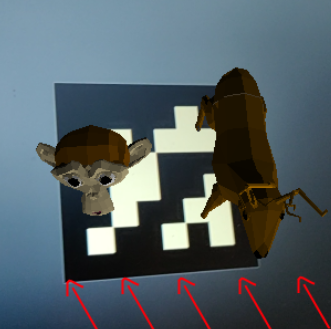
\includegraphics[scale=0.5]{img/flat_shading.png}
            \caption{Ombrage plat sur les objets à partir d'une source lumineuse représentée par les flèches rouges}
        \end{figure}

    \section{Projection et caméra}

        \subsection{Calibration}
        
        \subsection{Projection}
